\documentclass[a4paper, 12pt]{article}
\usepackage[brazil]{babel}
\usepackage[utf8]{inputenc}
\usepackage{amsmath}
\usepackage{indentfirst}
\usepackage{graphicx}
\usepackage{multicol,lipsum}
\usepackage[a4paper, top=3cm, left=3cm, bottom=3cm, right=3cm]{geometry}
\usepackage{setspace}
\usepackage{multirow}
\usepackage{float}
\usepackage[table]{xcolor}
%\usepackage{pdflscape}
\usepackage[DIV=15]{typearea}
\usepackage[nottoc]{tocbibind}
\usepackage[sort,numbers]{natbib}
%\usepackage{cite}

\documentclass[letterpaper]{article}

% bib pack %%%%%%%%%%%%%%%%%%%%%%%%%%%%%%%%%%%%%%%%%%%%%%%%%%%%%%%%%%%%%%%%%%%%%
\usepackage[utf8]{inputenc}
\usepackage{geometry}
    \geometry{left=3cm,right=2cm,top=2cm,bottom=2cm}
%
\usepackage[spanish]{babel}
%
\usepackage[fixlanguage]{babelbib}
    \bibliographystyle{babunsrt}
%
\usepackage{url}

\begin{document}
	
\onehalfspacing
\setlength{\parindent}{1.25cm}

\begin{titlepage}
	\begin{center}
	
		\large{PONTIFÍCIA UNIVERSIDADE CATÓLICA DO RIO DE JANEIRO}\\
		\large{DEPARTAMENTO DE ENGENHARIA MECÂNICA}\\ 
		\large{ENG1784 - AUTOMACAO DA MANUFATURA}\\
		
	\begin{figure}[!ht]
	\centering
	
\includegraphics[scale=1]{brasao.png}
	\end{figure}
		
        \vspace{10pt}
        \textbf{\LARGE{INTERTRAVAMENTO DA PONTE ROLANTE COM A LINHA DE MONTAGEM}}\\
		\vspace{1,5cm}
		ALUNOS:\\ 
		Carlos Andrés Abanto Tirado - 1910291 \\
		Matheus Barros Freires - 1813105 \\
		Paloma Fernanda Loureiro Sette - 1621595\\
		Rodrigo Lazzarotto - 1811514\\
		Wallace Matias Felix de Paiva - 1813173 \\
		
		\vspace{3cm}
		Rio de Janeiro, abril de 2022
	\end{center}

\end{titlepage}

\newpage
\pagenumbering{roman}
\tableofcontents

\newpage
\listoffigures

\newpage
\pagenumbering{arabic}
\setcounter{page}{1}

\newpage
\section{Introdução}
A empresa de manutenção de turbinas aeronáuticas X possui um galpão, onde se realiza o processo de desmontagem das peças. Dessa maneira, conta com uma ponte rolante para transportar e distribuir as turbinas para três linhas de desmontagem. Além disso, estão presentes talhas interligadas, responsáveis por içar a peça e que se deslocam por um trilho central, assim como ferramentas para a ancoragem das peças, que são sustentadas por outros dois trilhos laterais.

\begin{figure}[H]
    \centering
    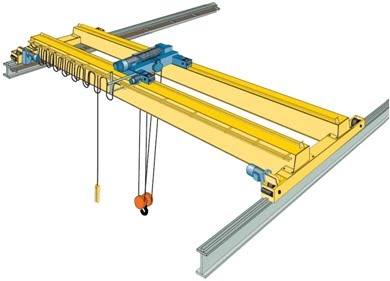
\includegraphics[width=9cm]{ponteRolante.jpeg}
    \caption{Ponte rolante}
\end{figure}

A ponte rolante é acionada pelo operador por meio de uma botoeira, na qual estão há botões de modo manual/automático, além de botões de anda e volta, que regulam o movimento da ponte ao ser ou não acionados.\par
Por sua vez, as talhas interligadas são controladas por uma botoeira que permite escolher entre modo manual ou automático, o que controla se seus movimentos serão individuais ou em conjunto. Ademais, cada talha tem seu movimento acionado por quatro botões: sobe, desce, anda e volta.\par
Desse modo, a ponte e as talhas possuem duas velocidades, sendo reguladas pela pressão exercida nos botões de acionamento de ambas, de forma que ao pressionar um pouco a velocidade é baixa e empurrando o botão a velocidade é alta.

\newpage
\section{Apresentação da problemática}

O desenvolvimento deste projeto baseia-se na necessidade de instalação de ponte rolante na entrada do galpão da linha de desmontagem da companhia X, possibilitando o transporte e distribuição das turbinas para um das 3 linhas de desmontagem. Ainda que o projeto mecânico já esteja desenvolvido, nos encarregamos de produzir o projeto de automação para tal.

Antes de realizar a instalação, devemos verificar uma série de fatores para decidir qual a maneira mais conveniente de fazer o serviço, bem como o modelo dos respectivos componentes a serem utilizados. Para uma montagem adequada, é necessário o conhecimento de algumas características a serem observadas, como o espaço em que o equipamento estará situado, pois a montagem muda de acordo com a área disponível, uma vez que existem espaços maiores e mais reduzidos. Logo, teremos que decidir quais os melhores acessórios para a instalação junto ao equipamento, de forma a garantir seu melhor uso e total produtividade.

\newpage
\section{Proposta de solução}

A proposta de solução irá tratar das problemáticas citadas anteriormente, focando na automação e segurança do projeto: O processo de alinhamento, que será abordado a utilização do sensores e sua utilização para o alinhamento da ponte, o processo de travamento da ponte para a linha, a fim de impedir que não ocorra a situação onde a ponte saia do seu alinhamento durante a utilização das talhas, e por fim, o travamento das rodas das talhas, para que não haja movimento das talhas que possa desprende-las da ponte.

\subsection{Processo de alinhamento}

Para o processo de automação do alinhamento da ponte rolante, será necessário a utilização de sensores que possam fornecer os dados necessários para esse processo, como a distância da ponte até onde ela deve ser posicionada para o descarregamento da turbina nas linhas de montagem.
O sensor escolhido foi AMS 300i 120, produzido pela Leuze Electronic LTDA, vide \ref{sensor}. 

\begin{figure}[H]
    \centering
    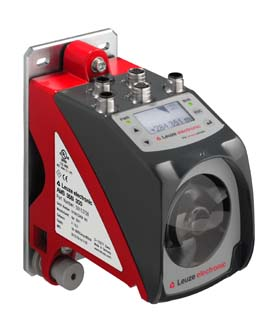
\includegraphics[width=6cm]{sensor.png}
    \caption{Sensor}
    \label{sensor}
\end{figure}
%\newpage

Sendo um sensor óptico de posicionamento, que funciona através do princípio do tempo de propagação da luz irradiada pelo sensor. A luz emitida pelo sensor se choca com um refletor, e, através do tempo de propagação da luz, calcula a distância do refletor para o sensor. O refletor será acoplado na ponte rolante, enquanto o sensor pode ser preso à parede de frente para a ponte. Tendo em conta que a distância máxima do refletor para o sensor não pode passar de 300 metros, não haverá problemas na utilização desse sensor no ambiente, além do fato de ser um sensor desenvolvido e adaptado para funcionar em pontes rolantes, onde há o movimento do corpo a ser calculado a distância.

Quanto ao detalhamento do processo de alinhamento: Uma vez que a ponte rolante começar a se locomover, o sensor óptico irá constantemente calcular a distância da ponte, esses dados da distância serão fornecidos a um CLP (Controlador Lógico Programável), que por sua vez fará o trabalho para que a determinada distância a velocidade da ponte mude para uma mais baixa, e quando já estiver perto da linha de montagem desejada, a ponte começará a parar até que esteja alinhada com a linha de montagem. Sabendo que o sensor utilizado possui uma precisão de 2 milímetros em sua medição, pode-se afirmar que o processo de alinhamento ocorrerá sem grandes imprecisões do sensor. A Figura \ref{excontrol}  mostra um exemplo de uma conexão entre o sensor e um controlador.

\begin{figure}[H]
    \centering
    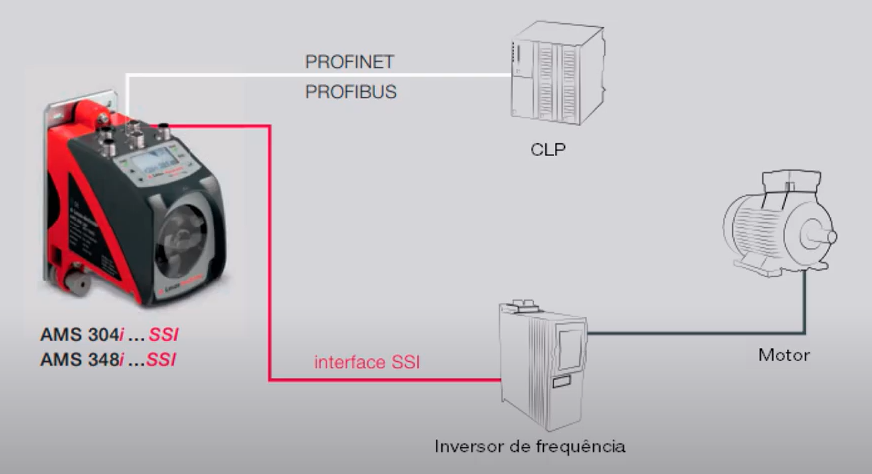
\includegraphics[width=11cm]{ExControl.png}
    \caption{Sensor e controlador}
    \label{excontrol}
\end{figure}


\subsection{Processo de intertravamento da ponte rolante com linha de montagem}

Após o alinhamento da ponte, é acionado um sistema de travamento entre ela e a linha de montagem, não permitindo que haja deslocamento indesejado durante o movimento das talhas. O intertravamento é realizado impedindo que o carro se mova em relação a viga de apoio, quando se encontra alinhado e parado a linha de montagem.

O sistema é composto mecanicamente por cilindros pneumáticos acoplados na base do carrinho (por meio de parafusos) e sapatas fixadas na ponta do pistão. É escolhido esse mecanismo pela facilidade na lógica de funcionamento. Se tratando do uso de cilindros pneumáticos, não é necessário grandes espaços para o armazenamento do gás, além de não ter gotejamento em casos de vazamentos. Junto a isso, o gás utilizado é o ar, inibindo preocupações ambientais.  

O acionamento do pistão é orientado ao funcionamento do compressor que controla a pressão do gás comprimido. Este compressor fica localizado fora da ponte rolante, não sendo colocado em perspectiva no desenho esquemático, e sua conexão com o cilindro é feito por cabos. Com o CLP, usando os mesmo dados do sensor da etapa de alinhamento, é orientado o funcionamento do compressor.

Na Figura \ref{travap} é apresentado a localização do sistema. Em cada ponta da base do carrinho terá um conjunto de trava para conferir garantia do funcionamento e estabilidade da movimentação.

\begin{figure}[H]
    \centering
    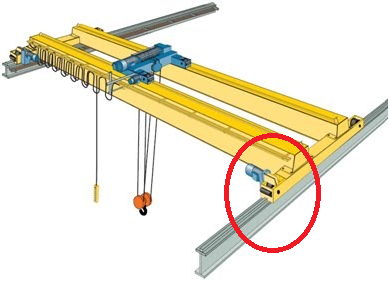
\includegraphics[width=10cm]{LocalTravaCarrinho.png}
    \caption{Posicionamento da trava}
    \label{travap}
\end{figure}

Na Figura \ref{Desenho} é apresentado um esquemático do conjunto de trava. Quando acionado, o pistão pressiona a sapata a viga, travando por meio do atrito e não permitindo deslizamento do carrinho.

\begin{figure}[H]
    \centering
    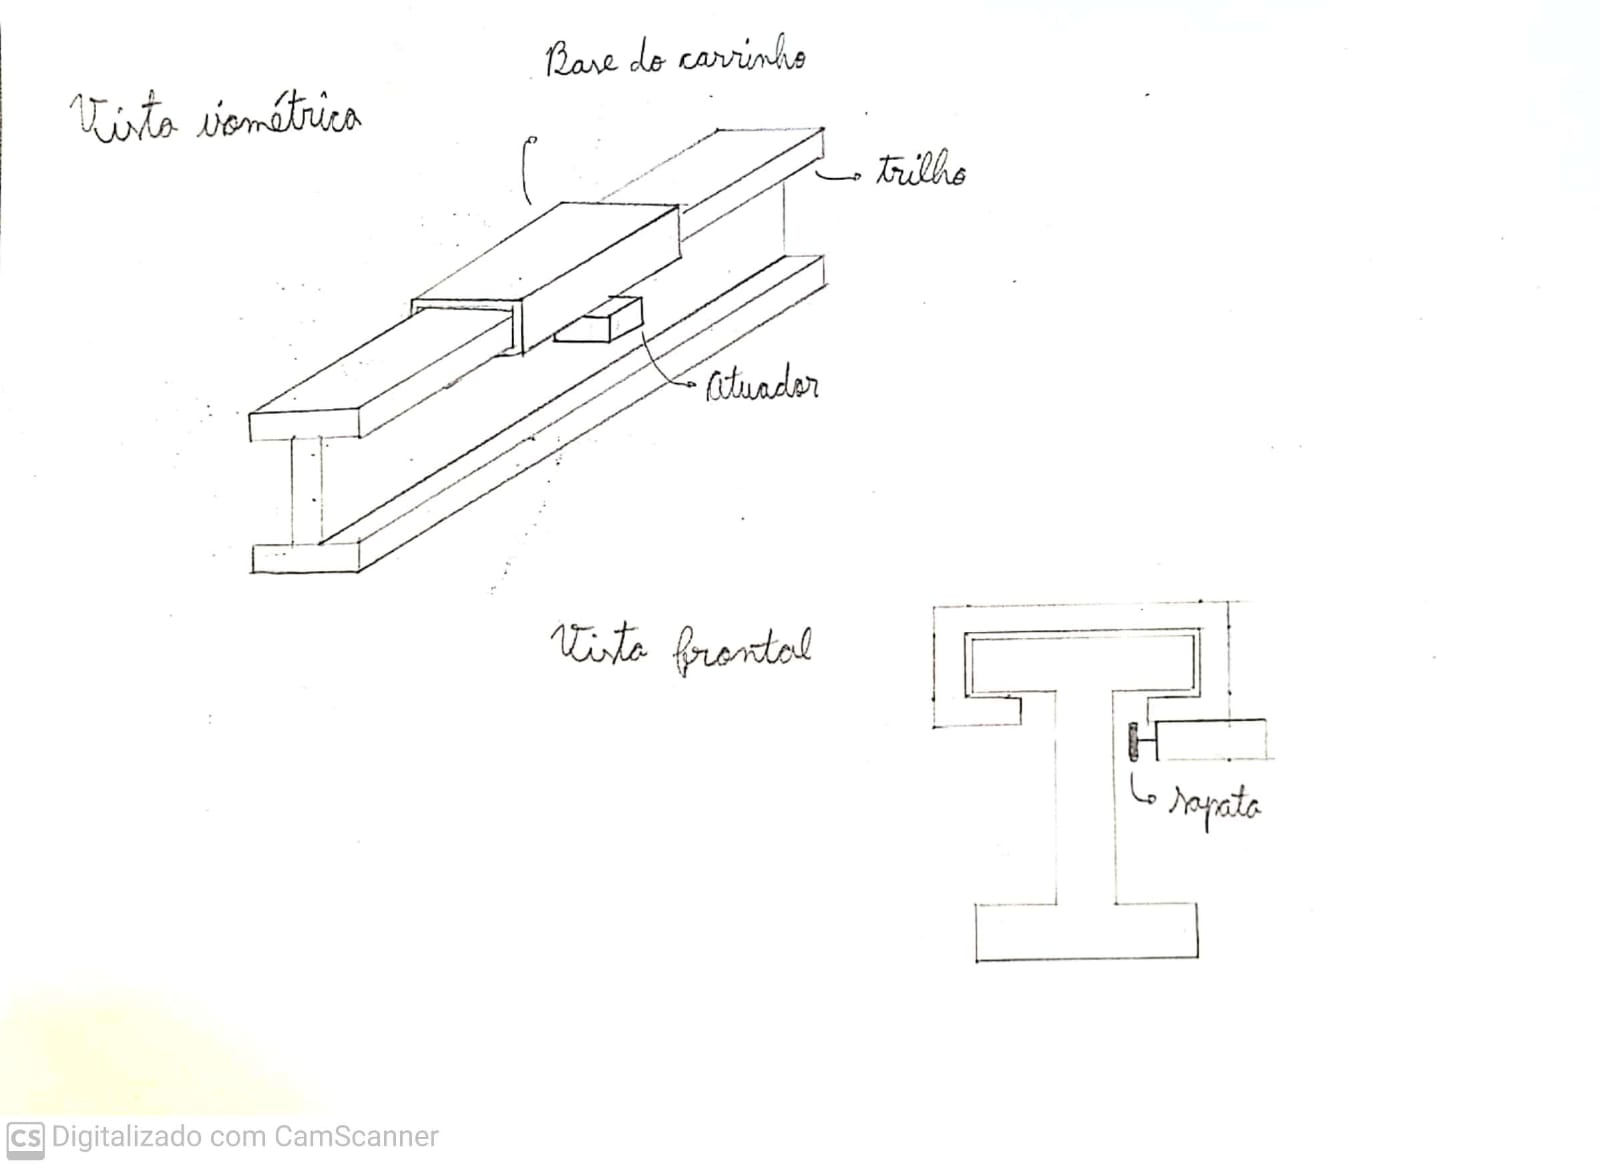
\includegraphics[width=12cm]{desenhoTravaCarrinho.jpeg}
    \caption{Esquemático do sistema de travamento do carrinho}
    \label{Desenho}
\end{figure}

\newpage
\subsection{Processo de travamento da roda das talhas}

Para evitar que as talhas saiam do trilho da ponte rolante enquanto não há alinhamento e intertravamento com uma das linhas de montagem, é necessário criar um mecanismo que, mesmo com o comando do operador, as talhas sejam barradas do lado direito e do lado esquerdo da viga central.

Como as linhas de montagem estão localizadas à esquerda das vigas da ponte rolante, a solução para o lado direito será um batente fixado na própria viga por solda. Já para o lado esquerdo, deverá ser colocado um mecanismo que pode liberar ou limitar o movimento das talhas e uma estrutura que suporte esse mecanismo.

O mecanismo será composto por dois motores DC e dois conjunto de engrenagens do tipo pinhão e cremalheira. O pinhão será ativado pelo motor, movimentando a cremalheira para frente e para trás. A função da cremalheira é servir de barreira para as talhas, que pode ser afastada através do acionamento pelo motor DC. Para que essa função seja realizada, será construída uma estrutura de aço para suportar a possível força da talha contra a cremalheira e para sustentar o mecanismo sobre a viga. A Figura \ref{conjp} mostra uma representação de um conjunto pinhão – cremalheira.


\begin{figure}[H]
    \centering
    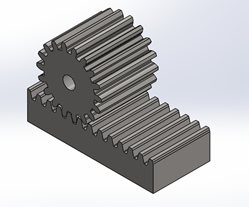
\includegraphics[width=9cm]{engrenagem.png}
    \caption{Conjunto pinhão - cremalheira}
    \label{conjpinha}
\end{figure}

A estrutura será presa na parte superior da viga, aparafusada para evitar grandes deformações na região central. Para amenizar deformações por momento fletor, um tipo de mão francesa será instalada entre a parte horizontal e a parte vertical. A parte vertical terá uma abertura para que caiba o conjunto pinhão cremalheira. Para sustentar o motor, uma extensão será instalada na parte vertical, assim como um furo para ligar o eixo do pinhão ao motor. Um croqui mostrando o mecanismo e duas vistas deste preso na viga central da ponte rolante está presente na Figura \ref{croqui}.

\begin{figure}[H]
    \centering
    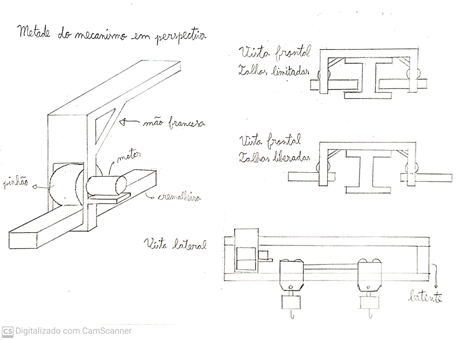
\includegraphics[width=9cm]{croqui.png}
    \caption{Croqui}
    \label{croqui}
\end{figure}

Enquanto não houver alinhamento e intertravamento da ponte com alguma das linhas, o mecanismo permanecerá parado, com a cremalheira barrando o movimento das talhas para a esquerda. Quando o sistema de controle detectar que o intertravamento foi concluído, ocorrerá a ativação do motor, movimentando o conjunto de engrenagens de modo a liberar o movimento das talhas para a esquerda. 

\newpage
\section{Conclusão}

Dado a problemática do sistema é desenvolvido uma solução que, alinhado ao funcionamento do sistema inicial da ponta, possibilita o intertravamento automatizado entre ela e qualquer linha de montagem presente. Além disso, confere maior segurança no uso do sistema, tal qual os travamentos do carrinho e das talhas, diminuindo possíveis riscos de acidentes.



% REFERENCIAS %%%%%%%%%%%%%%%%%%%%%%%%%%%%%%%%%%%%%%%%%%%%%%%%%%%%%%%%%%%%%%
    \nocite{*}
    \bibliography{src/sample}
    
\end{document}
\section{Referências Bibliográficas}

\end{document}
